%%%%%%%%%%%%%%%%%%%%%%%%%%%%%%%%%%%%%%%%%
% Golang Reference Sheet
% Version 0.1 (01/09/2016)
%
% Author:
% Andy Walker (https://github.com/alaska)
% License:
% The MIT License (see included LICENSE file)
%
%%%%%%%%%%%%%%%%%%%%%%%%%%%%%%%%%%%%%%%%%

% Basic document setup
\documentclass[10pt]{article}
%\usepackage{lua-visual-debug}
\usepackage[portrait, margin=0.25in]{geometry}
\setlength{\parindent}{0pt}
\usepackage{inconsolata}
\usepackage[T1]{fontenc}
\renewcommand*\familydefault{\ttdefault} %% Only if the base font of the document is to be typewriter style
\usepackage{luatexja} %% Japanese text

% Local imports (and anything they include) first
\usepackage{import}
% To allow us to use solarized colors elsewhere in the document
\subimport{theme/}{solarized}

% Package imports
\usepackage{booktabs}
\usepackage{multirow}
\usepackage[outputdir=\directlua{tex.sprint(os.getenv('BUILD_DIR'))}]{minted}
\usepackage{tcolorbox}
\usepackage{pdfrender}
\usepackage[fleqn]{amsmath}

% Fix Minted spacing
\newlength{\fancyvrbtopsep}
\newlength{\fancyvrbpartopsep}
\makeatletter
\FV@AddToHook{\FV@ListParameterHook}{\topsep=\fancyvrbtopsep\partopsep=\fancyvrbpartopsep}
\makeatother
\setlength{\fancyvrbtopsep}{-3pt}
\setlength{\fancyvrbpartopsep}{0pt}

% Frame/box definitions
%\pagecolor{sbase01}
%TODO: Look at sidebyside, overlay, tcbline, segmentation style
\newtcolorbox{codebox}[1][]{fontupper=\scriptsize\texttt, coltext=black, colback=sbase3, fonttitle=\scriptsize\texttt, coltitle=white, colbacktitle=sblue, arc=3pt, boxrule=0pt, titlerule=0.5pt, box align=top, before skip=0pt, after skip=3pt, left skip=0pt, right skip=3pt, toptitle=3pt, bottomtitle=3pt, subtitle style={after skip=6pt}, boxsep=0pt, left=3pt, top=3pt, halign=left, title=#1}

% Code formatting alias/options
\usemintedstyle{solarizedlight}
\newminted{go}{autogobble}

% Custom commands
\newcommand*{\CheapShadow}[1]{%
  \begingroup
    \leavevmode
    \rlap{\kern.3pt\raise-.3pt\hbox{%
      \pdfrender{
        TextRenderingMode=FillStroke,
        LineWidth=.2pt,
        StrokeColor=black,
		FillColor=black,
      }#1%
    }}%
    \rlap{%
      \pdfrender{
        TextRenderingMode=Stroke,
        LineWidth=.2pt,
      }#1%
    }%
    \hbox{#1}%
  \endgroup
}

\begin{document}
\begin{minipage}{\textwidth}
    \fontfamily{pag}%
    \fontseries{b}%
    \textcolor{sblue}{\CheapShadow{\Large{Go Quick Reference}\tiny{version $\alpha$}}}\hfill
    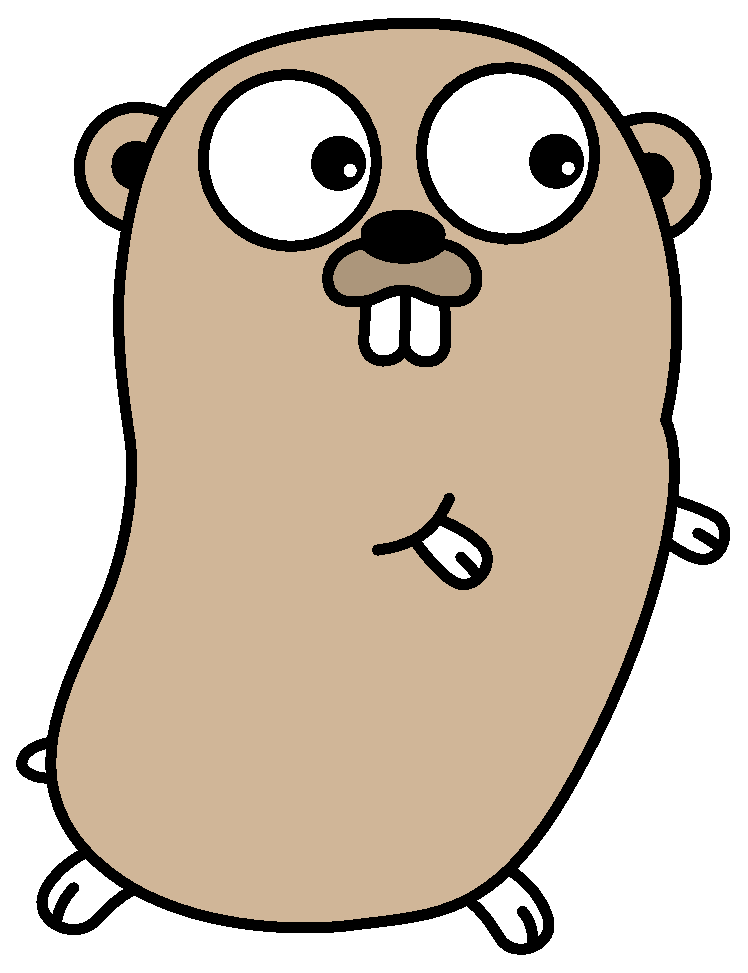
\includegraphics[width=0.5cm]{./figures/gopher.eps}
\end{minipage}
\begin{minipage}[t]{.25\textwidth}
    \begin{codebox}[Operators]
        \setlength{\tabcolsep}{2pt}%
        \begin{tabular}{@{}l|llllllll@{}}
            Unary & +  & -  & \textasciicircum &&&&&\multirow{6}*{\rotatebox[origin=c]{270}{$\underrightarrow{precedence}$}}\\
            Multiplication & * & / & \% & << & >> & \& & \&\textasciicircum&\\
            Addition & + & - & | & \textasciicircum &&&&\\
            Comparison & == & != & < & <= & > & >= &&\\
            Logical & \&\& &&&&&&&\\
                    & ||   &&&&&&&
        \end{tabular}%
    \end{codebox}
	\begin{codebox}[Structure - Exectutable]
        \begin{gocode}
            package main
            import (
                "pkg"
                "pkg2"
            )
            import "fmt" //or one per-line

            const (
                numberOne = 1
            )
            const hello = "Hello, 世界"

            //main.main required for executable
            func main() {
                // Code
            }
		\end{gocode}
        \tcbsubtitle{Structure - Package}
        \begin{gocode}
            package mylib

            func CallMeFromOutside
        \end{gocode}
	\end{codebox}
    \begin{codebox}[Intro]
        \begin{gocode}
            package main
            import (
            "fmt"
            )
            func main() {
                a := 1 + 2
                b := false
                "foo goto bar"
                5-3
                "5-3"
                5*3
            }
        \end{gocode}
    \end{codebox}
    \begin{codebox}[More]
        %\inputminted[firstline=2,lastline=10]{go}{./go/quickref_src.go}
        \begin{gocode}
            func foo(bar int, baz int) int {
                return bar + baz
            }
        \end{gocode}
    \end{codebox}
    \begin{codebox}[more2]
        \begin{gocode}
            func foo(bar int, baz int) int {
                return bar + baz
            }
        \end{gocode}
    \end{codebox}
    \begin{codebox}
        \begin{gocode}
            package anothermain
            import (
            "fmt"
            )
            func main() {
                fmt.Println("Gopher, save me")
            }
        \end{gocode}
    \end{codebox}
\end{minipage}%
\begin{minipage}[t]{.25\textwidth}
    \begin{codebox}
        \begin{gocode}
            package anothermain
            import (
            "fmt"
            )
            func main() {
                fmt.Println("Gopher, save me")
            }
        \end{gocode}
    \end{codebox}
\end{minipage}%
\begin{minipage}[t]{.25\textwidth}
    \begin{codebox}
        \begin{gocode}
            package anothermain
            import (
            "fmt"
            )
            func main() {
                fmt.Println("Gopher, save me")
            }
        \end{gocode}
    \end{codebox}
\end{minipage}%
\begin{minipage}[t]{.25\textwidth}
    \tcbset{right skip=0pt}%
    \begin{codebox}
        \begin{gocode}
            package anothermain
            import (
            "fmt"
            )
            func main() {
                fmt.Println("Gopher, save me")
            }
        \end{gocode}
    \end{codebox}
\end{minipage}%
\end{document}
